\documentclass{article}
\usepackage{polski}
\usepackage[utf8]{inputenc}
\usepackage{graphicx}
\usepackage{amsmath}
\usepackage{float}
\usepackage{tikz}
\usepackage{csvsimple}
\title{Sprawozdanie}
\author{Kajetan Bilski 244942}

\begin{document}
	\maketitle
	\pagenumbering{arabic}
\section{Zadanie 1.}
W tym zadaniu trzeba powtórzyć operacje z zadania 5. na poprzedniej liście ze zmienionymi danymi i wyniki porównać z oryginalnymi.
\begin{table}[h!]
  \begin{center}
    \caption{Float32}
    \label{tab:table1}
    \begin{tabular}{r|c|c}
      & \textbf{Stare wyniki} & \textbf{Nowe wyniki}\\
      \hline
      \textbf{W przód} & -0.4999443 & -0.4999443\\
      \textbf{W tył} &  -0.4543457 & -0.4543457\\
      \textbf{Od największego do najmniejszego} & -0.5 & -0.5\\
      \textbf{Od najmniejszego do największego} & -0.5 & -0.5\\
    \end{tabular}
  \end{center}
\end{table}
\begin{table}[H]
	\begin{center}
		\caption{Float64}
		\label{tab:table2}
		\begin{tabular}{r|c|c}
			& \textbf{Stare wyniki} & \textbf{Nowe wyniki}\\
			\hline
			\textbf{W przód} & 1.0251881368296672e-10 & -0.004296342739891585\\
			\textbf{W tył} & -1.5643308870494366e-10 & -0.004296342998713953\\
			\textbf{Od największego do najmniejszego} & 0.0 & -0.004296342842280865\\
			\textbf{Od najmniejszego do największego} & 0.0 & -0.004296342842280865\\
		\end{tabular}
	\end{center}
\end{table}
Jak widać o ile nieznaczna zmiana danych wpływa na wynik dla Float64, to przez mniejszą ilość bitów mantysy w Float32 różnica ta zostaje zgubiona w trakcie obliczeń.
%\newpage
\section{Zadanie 2.}
W tym zadaniu trzeba użyć 2 różnych programów do wizualizacji, żeby narysować wykresy podanej funkcji $f(x) = e^x*ln(1+ e^{-x})$, policzyć jej faktyczną granicę i stwierdzić przyczynę rozbieżności. Do wykresów użyłem Wolframa Alpha i Julia Plots.
\begin{figure}[H]
	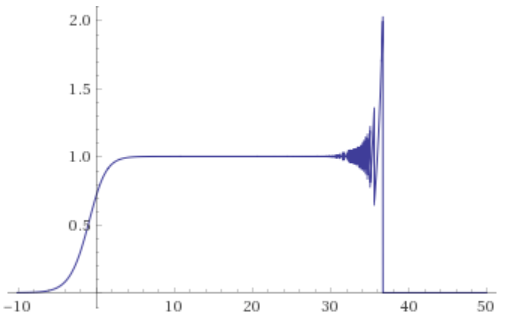
\includegraphics[width=\linewidth]{wolfram-wykres.png}
	\caption{Wykres wygenerowany przez Wolfram Alpha.}
	\label{fig:wolfram}
\end{figure}
\begin{figure}[H]
	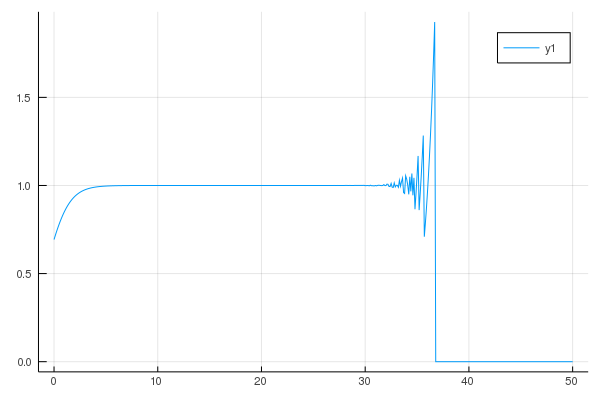
\includegraphics[width=\linewidth]{wykres.png}
	\caption{Wykres wygenerowany przez Julia Plots.}
	\label{fig:julia}
\end{figure}
Z reguły de l'Hospitala możemy wyliczyć, że:
\[ \lim_{x \to \infty} f(x) = \lim_{x \to -\infty} \frac{ln(1+e^x)}{e^x} = \lim_{x \to -\infty} \frac{\frac{e^x}{1+e^x}}{e^x} = \lim_{x \to -\infty} \frac{1}{1+e^x} = 1 \]
\newline
Widać to na wykresie do pewnego momentu.
\section{Zadanie 3.}
W tym zadaniu trzeba obliczyć błędy względne dla różnych metod wyliczania (gaussa i z inwersją) wektora x dla różnych macierzy (hilberta i losowych z ustalonym uwarunkowaniem).
\begin{figure}[H]
	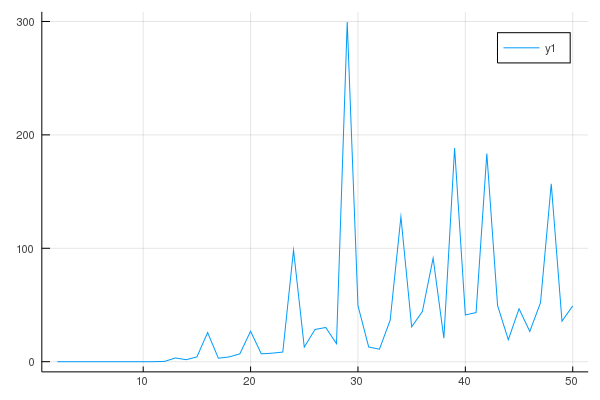
\includegraphics[width=\linewidth]{hilbert_gauss.png}
	\caption{Wykres pokazuje zależność błędu względnego od stopnia macierzy Hilberta dla eliminacji Gaussa.}
	\label{fig:hilbert-gauss}
\end{figure}
\begin{figure}[H]
	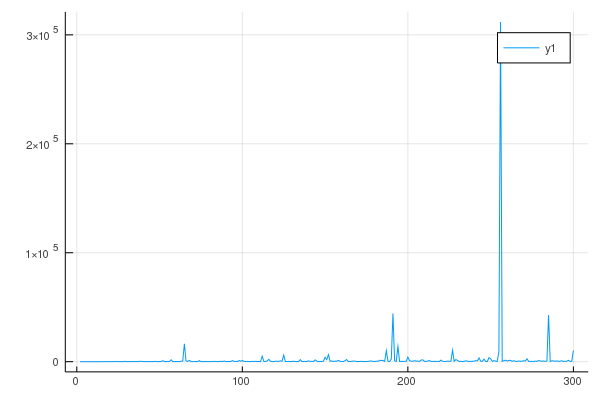
\includegraphics[width=\linewidth]{hilbert_inwersja.png}
	\caption{Wykres pokazuje zależność błędu względnego od stopnia macierzy Hilberta dla metody z inwersją.}
	\label{fig:hilbert-inv}
\end{figure}
\begin{table}[H]
	\begin{center}
		\begin{tabular}{r|l|l}
			\bfseries Stopień macierzy & \bfseries Wskaźnik uwarunkowania & \bfseries Błąd względny
			\\\hline
			\csvreader[head to column names]{matcond_gauss.csv}{}
			{\\\n & \c & \val}
		\end{tabular}
		\caption{Średni błąd względny dla macierzy losowych i eliminacji Gaussa.}
	\end{center}
\end{table}
\begin{table}[H]
	\begin{center}
		\begin{tabular}{r|l|l}
			\bfseries Stopień macierzy & \bfseries Wskaźnik uwarunkowania & \bfseries Błąd względny
			\\\hline
			\csvreader[head to column names]{matcond_inwersja.csv}{}
			{\\\n & \c & \val}
		\end{tabular}
		\caption{Średni błąd względny dla macierzy losowych i metody z inwersją.}
	\end{center}
\end{table}
\section{Zadanie 4.}
W tym zadaniu trzeba użyć Julii z pakietem Polynomials do policzenia pierwiastków wielomianu Wilkinsona $z_{k}$, $1\leq k\leq 20$, a następnie sprawdzić ich odchył prawdziwych pierwistków tego wielomianu. Na końcu trzeba powtórzyć eksperyment z lekko zmienionym drugim współczynnikiem wielomianu.
\begin{table}[H]
	\begin{center}
		\begin{tabular}{r|c|c|c}
			\bfseries $k$ & \bfseries $|P(z_{k})|$ & \bfseries $|p(z_{k})|$ & \bfseries $|z_{k}-k|$
			\\\hline
			\csvreader[head to column names]{zad4.csv}{}
			{\\\k & \P & \p & \diff}
		\end{tabular}
		\caption{Wyniki dla pierwiastków wyliczonych przez Julia Polynomials.}
	\end{center}
\end{table}
\begin{table}[H]
	\begin{center}
		\begin{tabular}{r|c}
			\bfseries $k$ & \bfseries $|P(z_{k})|$
			\\\hline
			\csvreader[head to column names]{zad4_wilkinson.csv}{}
			{\\\k & \P}
		\end{tabular}
		\caption{Wyniki dla zaburzonego wielomianu.}
	\end{center}
\end{table}
\section{Zadanie 5.}
W tym zadaniu trzeba przeprowadzić ekperyment z modelem logistycznym, obliczając wartości kolejnych iteracji danego równania rekurencyjnego, dwa razy na Float32 (raz z obcięciem) i raz na Float64, a następnie porównać wyniki.
\begin{figure}[H]
	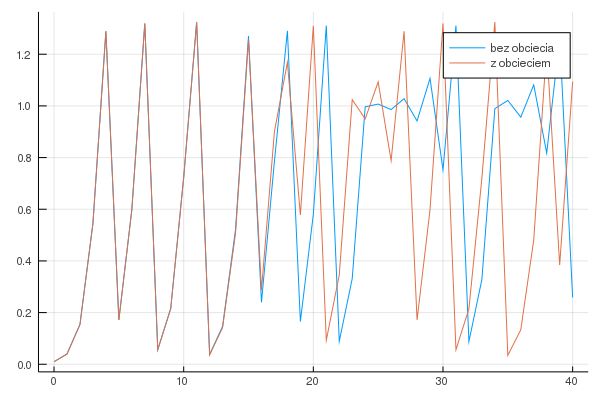
\includegraphics[width=\linewidth]{zad5_1.png}
	\caption{Porównanie wykresów dla Float32 z i bez obcięcia po 10. iteracji.}
	\label{fig:cut}
\end{figure}
\begin{figure}[H]
	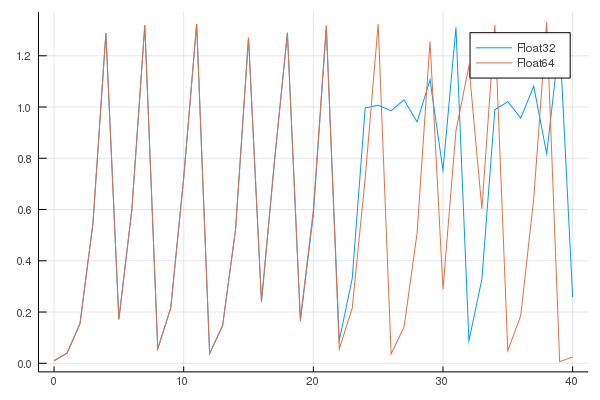
\includegraphics[width=\linewidth]{zad5_2.png}
	\caption{Porównanie wykresów dla Float32 i Float64.}
	\label{fig:floats}
\end{figure}
\section{Zadanie 6.}
W tym zadaniu trzeba przeanalizować zachowanie 7 ciągów stworzonych przez funkcję rekurencyjną $x_{n+1}=x_{n}^{2}+c$ dla podanych $x_{0}$ i $c$.
\begin{figure}[H]
	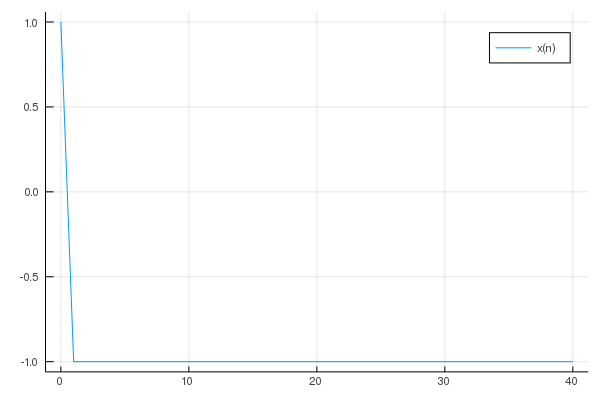
\includegraphics[width=\linewidth]{zad6_1.png}
	\caption{$c=-2$ i $x_{0}=1$}
	\label{fig:z61}
\end{figure}
\begin{figure}[H]
	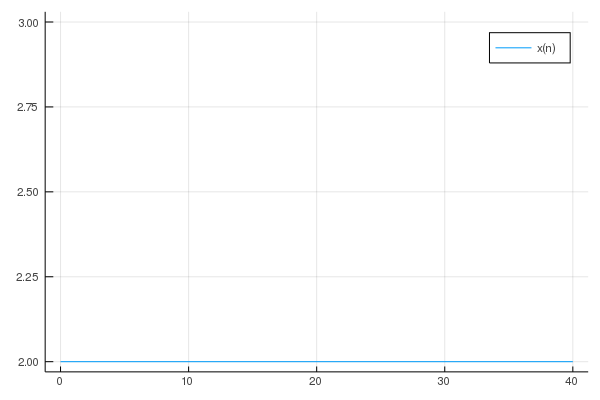
\includegraphics[width=\linewidth]{zad6_2.png}
	\caption{$c=-2$ i $x_{0}=2$}
	\label{fig:z62}
\end{figure}
\begin{figure}[H]
	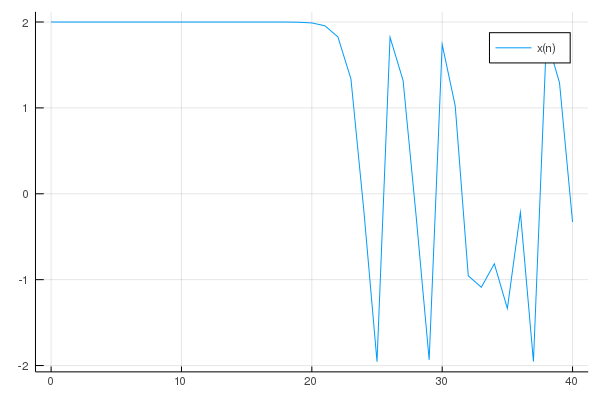
\includegraphics[width=\linewidth]{zad6_3.png}
	\caption{$c=-2$ i $x_{0}=1.99999999999999$}
	\label{fig:z63}
\end{figure}
\begin{figure}[H]
	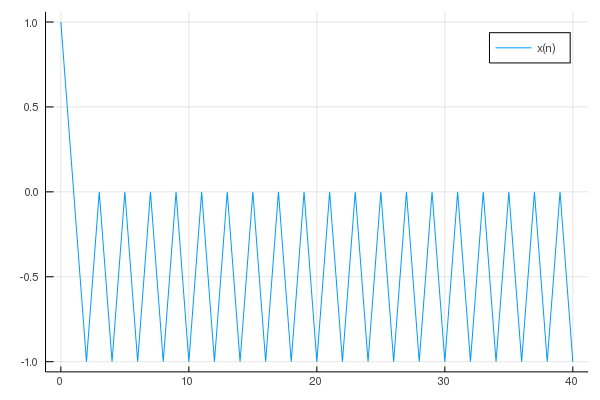
\includegraphics[width=\linewidth]{zad6_4.png}
	\caption{$c=-1$ i $x_{0}=1$}
	\label{fig:z64}
\end{figure}
\begin{figure}[H]
	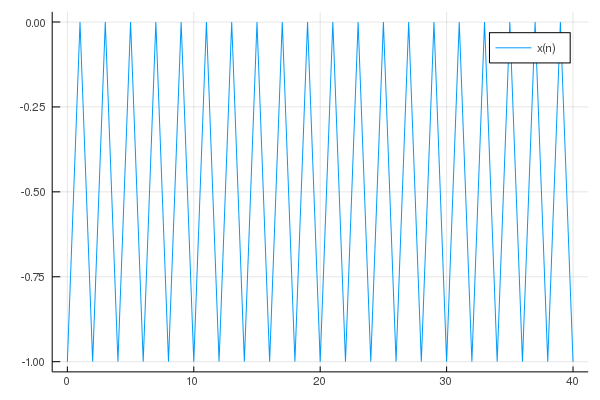
\includegraphics[width=\linewidth]{zad6_5.png}
	\caption{$c=-1$ i $x_{0}=-1$}
	\label{fig:z65}
\end{figure}
\begin{figure}[H]
	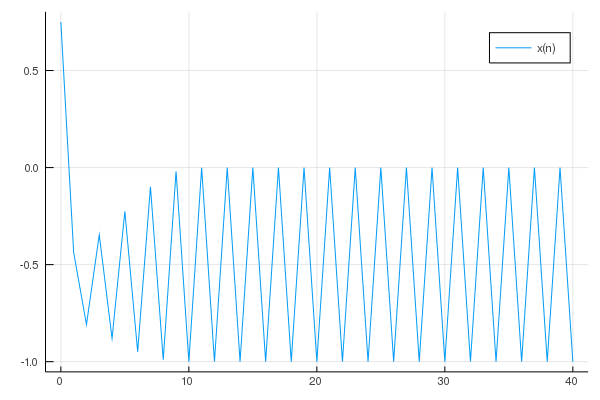
\includegraphics[width=\linewidth]{zad6_6.png}
	\caption{$c=-1$ i $x_{0}=0.75$}
	\label{fig:z66}
\end{figure}
\begin{figure}[H]
	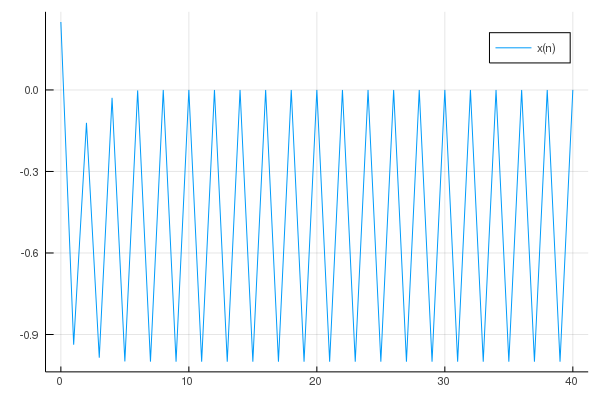
\includegraphics[width=\linewidth]{zad6_7.png}
	\caption{$c=-1$ i $x_{0}=0.25$}
	\label{fig:z67}
\end{figure}
\end{document}